\documentclass[11pt,aspectratio=1610,xcolor=dvipsnames]{beamer}

\usetheme[
    background=light,
    numbering=fraction,
    block=fill,
    progressbar=frametitle
]{metropolis}

\graphicspath{{img/}}

\usepackage[style=authortitle-ibid,backend=biber]{biblatex}
\addbibresource{refs.bib}
\setbeamerfont{footnote}{size=\scriptsize}

\usepackage{physics}
\usepackage{bbm}
\usepackage{booktabs}
\usepackage[most,skins,theorems]{tcolorbox}
\tcbset{variables/.style={colback=yellow!20,colframe=yellow}}
\usepackage{tikz}
\usetikzlibrary{shapes.geometric, arrows, shadows}
\usetikzlibrary{fit, backgrounds}



% \colorlet{LightLavender}{Lavender!40!}
\newtcolorbox{prob}{colback=red!5!white,colframe=red!75!black}
\usefonttheme[onlymath]{serif}
\usepackage{quantikz}
\usepackage{qrcode}
\usepackage{pgfplots}
\usepackage{pythonhighlight}

\newcommand{\R}{\mathbb{R}}
\newcommand{\U}[1]{\mathsf{U}(#1)}
\newcommand{\defeq}{\stackrel{\text{\tiny def}}{=}}

\titlegraphic{
\includegraphics[width=0.3\textwidth]{unitary_fund_logo.png}}

\title{Richardson Extrapolation}
\subtitle{Quantum Wednesday}
\date{Feb 8, 2023}
\author{Nate Stemen}


\begin{document}

\maketitle

\begin{frame}{Today's Paper}
	\begin{figure}[h]
		\centering
		
\includegraphics[width=0.9\textwidth]{abstract.png}
	\end{figure}
	\begin{center}
		\url{https://arxiv.org/abs/2201.08080}
	\end{center}
\end{frame}

\begin{frame}{Overview}
	\begin{enumerate}
		\item What is Richardson Extrapolation?
		\item How do we \emph{already} use it?
		\item What sort of optimizations do the authors find?
		\item Should we implement this?
	\end{enumerate}
\end{frame}

\begin{frame}{What is extrapolation?}

\end{frame}

\begin{frame}[fragile]{How do we use Richardson Extrapolation?}
	% \begin{noindent}
	\begin{python}
		class RichardsonFactory():
			def extrapolate(
				scale_factors: Sequence[float],
				exp_values: Sequence[float],
				full_output: bool = False,
			) -> ExtrapolationResult:
				# Richardson extrapolation is a particular case of a
				# polynomial fit with order equal to the number of
				# data points minus 1.
				order = len(scale_factors) - 1
				return PolyFactory.extrapolate(
					scale_factors, exp_values, order, full_output
				)
	\end{python}
	% \end{noindent}
\end{frame}

\begin{frame}{What could we optimize?}
	\begin{enumerate}
		\item Is there a way to reduce the increase in variance?
		\item Is there a scaling method for the $x_i$'s that optimizes the bias/variance tradeoff?
		\item Is there an optimal number of samples $n$?
	\end{enumerate}
\end{frame}

\begin{frame}
	\frametitle{Node Spacing}

	\begin{align*}
		x_j^\mathrm{L} & = 1 + j(x_1 - 1)                                                                             \\
		x_j^\mathrm{E} & = x_1^j                                                                                      \\
		x_j^\mathrm{C} & = 1 + \frac{\sin^2(\frac{j}{n}\frac{\pi}{2})}{\sin^2(\frac{1}{n}\frac{\pi}{2})}(x_1 - 1)     \\
		x_j^\mathrm{T} & = 1 + \frac{\sin^2(\frac{j}{n+1}\frac{\pi}{2})}{\sin^2(\frac{1}{n+1}\frac{\pi}{2})}(x_1 - 1)
	\end{align*}
	\begin{figure}[h]
		\centering
		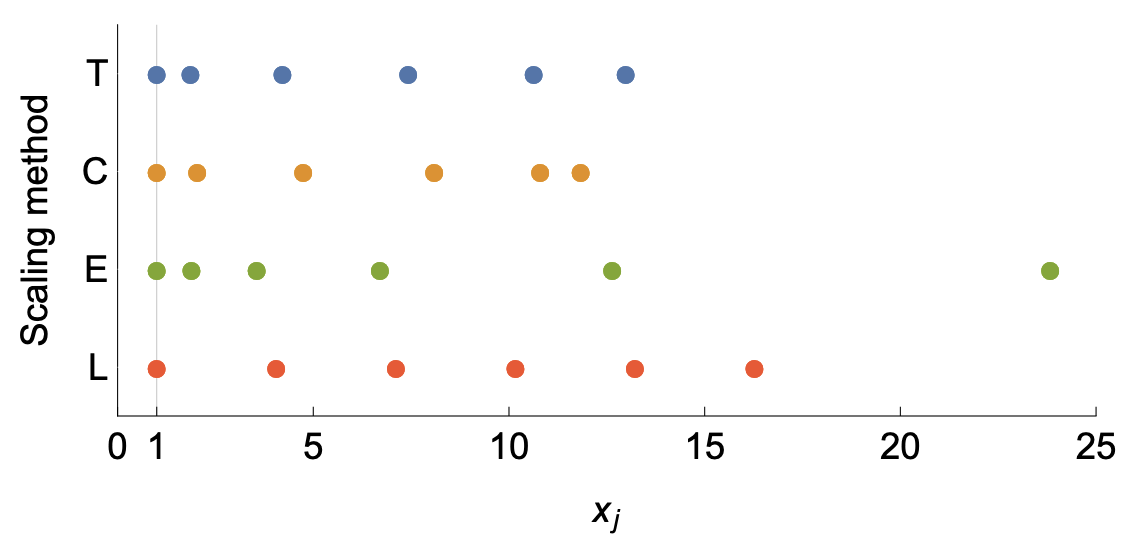
\includegraphics[width=0.5\textwidth]{spacing.png}
		\caption{<caption>}
		\label{<label>}
	\end{figure}

\end{frame}

% \begin{frame}{References}
% 	\nocite{*}
% 	\printbibliography[heading=none]
% \end{frame}

\begin{frame}[standout]
	Thank you!
\end{frame}

\end{document}
